\documentclass[lang=cn,11pt,a4paper]{elegantpaper}
\usepackage{algorithm}  
\usepackage{algorithmicx}  
\usepackage{algpseudocode}  
\usepackage{amsmath} 
\usepackage{makecell}
\floatname{algorithm}{算法}
\title{$\sin(x)$的数值求解与误差分析}
\author{自72 \quad 陈策 \quad 2017011619}
\date{\zhtoday}
\begin{document}
\maketitle
\tableofcontents
\clearpage
\section{任务介绍}
此次作业为数值分析课程的第二次大作业。
\subsection{题目简述}
使用计算机编程实现$\sin(x)$的数值求解并分析误差,输入为弧度值,考虑到特别大的输入对计算的储存精度要求太高,为避免复杂的数组计数形式,输入值的范围为$(-10,10)$,其有效数字为6位。
\subsection{题目要求}
\begin{enumerate}
  \item 采用逼近、数值积分、常微分方程中至少两种算法;
  \item 方法本身能够达到任意精度;
  \item 分析不同方法的方法误差以及存储误差对最终结果的影响;
  \item 分析比较选用方法的计算代价、收敛速度等;
  \item 具体计算结果至少精确到小数点后第4位;
  \item $\sin(x)$是周期函数,而且具有一定的对称性,同学们可以从这方面进行思考;
  \item 原则上只能使用可以进行误差分析的基础运算如加减乘除,其他的函数需要自己来实现,并考虑其误差;
  \item 在程序中可以使用$\pi,\ e, \ \sqrt{2}$之类的无理数, 但要考虑使用这些无理数带来的误差;
  \item 可以使用$\sin(x)$在特殊点上的值;
  \item 请尽量使用$C,\ C++,\ C\#$等编程语言,不要使用$MATLAB,\ Python$等脚本语言。
\end{enumerate}
\section{先决条件}
在实现任务要求前,由于对相关库的使用要求严格,笔者在完成任务时手动编写了如下计算函数,在本程序中设计数值计算部分的相关函数均为独立编写完成,对于GUI界面的美化使用了GitHub上的开源界面库\href{https://github.com/MaterialDesignInXAML/MaterialDesignInXamlToolkit}{MaterialDesignInXamlToolkit}。
\subsection{阶乘}
阶乘运算采用递归运算,详细算法参见\href{https://github.com/Antonio-Chan/SineCalculate}{源代码}。
\subsubsection{误差分析}
由于阶乘计算方法为阶乘的定义,所以方法误差可视为0,下面考虑由于计算机存储的限制导致的存储误差:

假定计算机存储变量的误差为$\Delta x$,理想的递归过程递推公式为
\begin{equation}
  f_{n}=n\cdot f_{n-1} 
\end{equation}
考虑存储误差有
\begin{equation}
  f_{n}=(n\pm \Delta x)\cdot(f_{n-1}\pm \Delta x)
\end{equation}
舍去高阶误差项得到
\begin{equation}
  \Delta f_n \leq |n+f_{n-1}|\cdot \Delta x \leq |f_n|\cdot \Delta x
\end{equation}
从而可以看出这种阶乘的计算方法会随着计算的数字的增大而成几何级数式的增加,可见此算法不适合计算大数阶乘,笔者使用$Double$类型存储变量,由于计算过程中数字不会超过$10^2$数量级,故此变量的最小精度为$1E-30$左右,在本任务中$|f_n|$不会超过$10! \approx 1E10$,所以阶乘计算的存储误差不会超过$1E-20$,此误差相对本任务极小,可以忽略。
\subsection{幂运算}
幂运算采用迭代运算,详细算法参见\href{https://github.com/Antonio-Chan/SineCalculate}{源代码}。
\subsubsection{误差分析}
由于阶乘计算方法为阶乘的定义,所以方法误差可视为0,下面考虑由于计算机存储的限制导致的存储误差:

假定计算机存储变量的误差为$\Delta x$,理想的迭代过程递推公式为
\begin{equation}
  f_{n}=k\cdot f_{n-1} 
\end{equation}
考虑存储误差有
\begin{equation}
  f_{n}=(k\pm \Delta x)^{n}
\end{equation}
舍去高阶误差项得到
\begin{equation}
  \Delta f_n = |(k\pm \Delta x)^{n}-k^n| \leq |n\cdot k^{n-1}|\cdot \Delta x
\end{equation}
从而可以看出这种求幂方式对于输入是比较敏感的,所以不适合较大的数的求幂计算,笔者使用$Double$类型存储变量,由于计算过程中数字不会超过$10^2$数量级,故此变量的最小精度为$1E-30$左右,在本任务中$|n\cdot k^{n-1}|$不会超过$10\cdot e^9 \approx 1E5$,所以阶乘计算的存储误差不会超过$1E-25$,此误差相对本任务极小,可以忽略。
\subsection{绝对值运算}
详细算法参见\href{https://github.com/Antonio-Chan/SineCalculate}{源代码}。
\subsubsection{误差分析}
由于绝对值运算方法为阶乘的定义,所以方法误差可视为0,下面考虑由于计算机存储的限制导致的存储误差:
假定计算机存储变量的误差为$\Delta x$,理想的绝对值运算公式为
\begin{equation}
  f(x)=|x|
\end{equation}
考虑存储误差有
\begin{equation}
  f(x)=|x\pm \Delta x|
\end{equation}
从而得到
\begin{equation}
  \Delta f(x)=|x\pm \Delta x|-|x| \leq \Delta x
\end{equation}
从而可以看出这种求绝对方式与输入数据大小无关,所以较为优良,笔者使用$Double$类型存储变量,由于计算过程中数字不会超过$10^2$数量级,故此变量的最小精度为$1E-30$左右,所以绝对值计算的存储误差不会超过$1E-30$,此误差相对本任务极小,可以忽略。
\subsection{平方根运算}
考虑到实际需要,由于$\sin(x)$的值域为$[-1,1]$,所以在处理过程中,需要开方的数字不超过$1$,所以简化了程序编写难度,笔者使用牛顿法求解平方根。
\subsection{原理解析}
假设方程$f(x)=0$有近似根$x_k$,假定$f'(x_k)\neq 0$,将函数$f(x)$在点$x_k$处展开
\begin{equation}
  f(x)\approx f(x_k)+f'(x_k)(x-x_k)
\end{equation}
则方程$f(x)=0$可近似表示为
\begin{equation}
  f(x_k)+f'(x_k)(x-x_k)=0
\end{equation}
于是可以得到牛顿法的不动点递推公式
\begin{equation}
  x_{k+1}=x_k-\frac{f(x_k)}{f'(x_k)}
\end{equation}
求某有理数$C$的平方根可等价为求以下方程的根
\begin{equation}
  f(x)=x^2-C=0
\end{equation}
其迭代函数为
\begin{equation}
  \phi(x)=\frac{x}{2}+\frac{C}{2x}
\end{equation}
根据迭代函数反复迭代并计算相邻两次迭代结果的差的绝对值,若小于给定精度则停止运算。
\subsection{算法流程}
算法流程参见\textbf{算法 1} 牛顿法求解平方根
\begin{algorithm}
  \caption{牛顿法求解平方根}
  \begin{algorithmic}
    \Require 待求数$C$与指定精度$\epsilon$
    \Ensure $C\in [0,1]$
    \begin{enumerate}
      \item 选定初始近似值$x_0=C$,计算$f_0=f(x_0)$,$f'_0=f'(x_0)$
      \item 根据迭代公式进行迭代计算下一项,$x_{k+1}=\phi(x_k)$
      \item 计算相邻两次结果差值的绝对值,并与给定精度进行比较,如果$|x_{k+1}-x_k|\leq \epsilon$则退出循环,返回数值$x_{k+1}$,否则继续执行上一步
    \end{enumerate}
  \end{algorithmic}
\end{algorithm}
\subsection{算法实现}
详细算法参见\href{https://github.com/Antonio-Chan/SineCalculate}{源代码}。
\subsection{程序框图}
\begin{figure}[htbp]
    \centering
    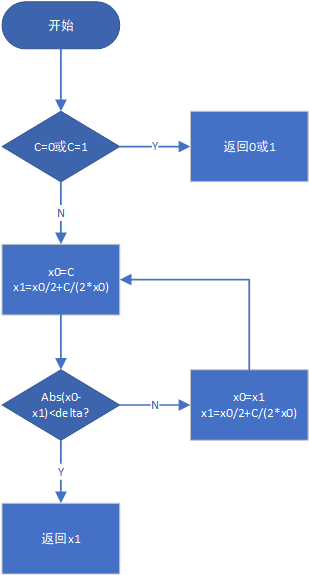
\includegraphics[width=0.45\linewidth]{src/A.png}
    \centering
    \caption{\textbf{算法 1} 牛顿法求解平方根}
\end{figure}
\subsection{误差分析}
\subsubsection{方法误差}
设$\Delta_n=x_n-\sqrt{C}$为第$n$步的方法误差:
\begin{equation}
  \Delta_{n+1}=\phi(x_n)-\phi(\sqrt{C})
\end{equation}
由泰勒展开知:
\begin{equation}
  \Delta_{n+1}=\leq (x_n-\sqrt{C})\phi'(\sqrt{C})+\frac{1}{2}(x_n-\sqrt{C})^2\phi''(\sqrt{C})=\Delta_n\phi'(\sqrt{C})+\frac{1}{2}\Delta_n^2\phi''(\epsilon)\quad \epsilon \in (x_n,\ \sqrt{C})
\end{equation}
由于
\begin{equation}
  \phi'(\sqrt{C})=0
\end{equation}
故
\begin{equation}
  \Delta_{n+1}\leq \frac{\max \left|\phi''(x)\right|}{2} \cdot \Delta_{n}
\end{equation}
得到
\begin{equation}
  \Delta_{n}\leq \frac{2}{\max \left|\phi''(x)\right|}\left(\frac{\max \left|\phi''(x)\right|}{2}\cdot (C-\sqrt{C})\right)^{2^n}
\end{equation}
又由于经过区间缩放之后,需开方的$x$在区间$[\frac{1}{2},\ 1]$
\begin{equation}
  \left|\phi''(x)\right| = \left|\frac{C}{x^3}\right|\leq \frac{1}{\sqrt{C}}\leq \sqrt{2}
\end{equation}
故方法误差为
\begin{equation}
  \Delta \leq \sqrt{2}\times(\frac{2-\sqrt{2}}{4})^{2^n}
\end{equation}
可见此误差极小。
\subsubsection{舍入误差}
设$\delta_n$为第$n$步的舍入误差,计算机贮存误差为$\delta_m$:
\begin{equation}
  \delta_{n+1}\leq \max\|\phi'(x)|\cdot \delta_n + \delta_m
\end{equation}
又由于经过区间缩放之后,需开方的$x$在区间$[\frac{1}{2},\ 1]$
\begin{equation}
  |\phi'(x)| = \left|\frac{1}{2}\left(1-\frac{C}{x^2}\right)\right| \leq \left|\frac{1}{2}\left(1-\frac{1}{C}\right)\right| \leq \frac{1}{2}
\end{equation}
得到
\begin{equation}
  \delta_{n+1}-2\delta_m \leq \frac{1}{2}(\delta_n - 2\delta_m)
\end{equation}
故
\begin{equation}
  \delta_{n} \leq \left(\frac{1}{2^{n-1}} + 2\right)\delta_m
\end{equation}
当$n$很大时,此误差与计算机存储误差相当。
\subsection{计算代价}
牛顿法的计算次数与指定精度和迭代函数有着密切联系,在本任务中,迭代次数不超过$10$
\subsection{收敛速度}
由于牛顿法的迭代函数为
\begin{equation}
  \phi(x)=x-\frac{f(x)}{f'(x)}
\end{equation}
求导得
\begin{equation}
  \phi '(x)=\frac{f(x)f''(x)}{[f'(x)]^2}
\end{equation}
其二阶导为
\begin{equation}
  \phi '(x)=\frac{f''(x)}{f'(x)}
\end{equation}
假定$x^*$是$f(x)$的一个单根,则
\begin{equation}
  \phi (x^*)=0,\quad \phi '(x^*)=0,\quad \phi ''(x^*)\neq 0
\end{equation}
从而得知牛顿法是二阶收敛的
\subsection{初值选取}
先证明本算法中的迭代公式对任意初值$x_0>0$都是收敛的,对迭代公式进行配方变换可得
\begin{equation}
  x_{k+1}-\sqrt{C}=\frac{1}{2\cdot x_k} (x_k-\sqrt{C})^2,\quad x_{k+1}+\sqrt{C}=\frac{1}{2\cdot x_k} (x_k+\sqrt{C})^2
\end{equation}
两式相除得
\begin{equation}
  \frac{x_{k+1}-\sqrt{C}}{x_{k+1}+\sqrt{C}}=\left(\frac{x_k-\sqrt{C}}{x_k+\sqrt{C}}\right)^2
\end{equation}
从而得到
\begin{equation}
  \frac{x_{k}-\sqrt{C}}{x_{k}+\sqrt{C}}=\left(\frac{x_0-\sqrt{C}}{x_0+\sqrt{C}}\right)^{2^k}
\end{equation}
整理得
\begin{equation}
  x_{k}-\sqrt{C}=2\sqrt{C}\cdot \frac{q^{2^k}}{1-q^{2^k}},\quad q=\frac{x_0-\sqrt{C}}{x_0+\sqrt{C}}
\end{equation}
对任意$x_0>0$总有$|q|<1$,故当$k\rightarrow \infty$时$x_k\rightarrow \sqrt{C}$,迭代过程对任意初值$x_0>0$都是收敛的,又由于对于任意$0\leq C \leq 1$有$0 \leq C \leq \sqrt{C} \leq 1$,所以选取$C$为初值是合理的。
\subsection{程序运行环境}
\begin{itemize}
  \item 运行平台:Windows10(1909)
  \item 开发环境:Visual Studio 2019
  \item 依赖框架:.NetFramework 4.7.2
\end{itemize}
双击可执行文件即可运行程序,如需源码编译,请根据\href{https://github.com/MaterialDesignInXAML/MaterialDesignInXamlToolkit}{MaterialDesignInXamlToolkit}要求安装GUI依赖包。
\subsection{区间转换}
为了避免误差分析中出现导致系数奇异的点,我们需要利用$sin(x)$的相关特性,对输入数据进行变换,将其变换到指定的区间中,此处我们将所有的输入变换到$[0,\ \frac{\pi}{2}]$上计算。

首先将输入数据对$2\pi$求模,将其转换到$[0,\ 2\pi)$区间,之后针对不同的$x'\in [0,\ 2\pi)$有如下分段计算函数:

$$\sin(x')=\sin(x'),\quad x'\in [0,\ \frac{\pi}{4})$$

$$\sin(x')=\cos(\frac{\pi}{2}-x')=\sqrt{1-\sin^2(\frac{\pi}{2}-x')},\quad x'\in [\frac{\pi}{4},\ \frac{\pi}{2})$$

$$\sin(x')=\sin(\pi -x')=\cos(x'-\frac{\pi}{2})=\sqrt{1-\sin^2(x'-\frac{\pi}{2})},\quad x'\in [\frac{\pi}{2},\ \frac{3\pi}{4})$$

$$\sin(x')=\sin(\pi -x'),\quad x'\in [\frac{3\pi}{4},\ \pi)$$

$$\sin(x')=-\sin(x'-\pi),\quad x'\in [\pi,\ \frac{5\pi}{4})$$

$$\sin(x')=-\sqrt{1-\sin^2(\frac{3\pi}{2}-x')},\quad x'\in [\frac{5\pi}{4},\ \frac{3\pi}{2})$$

$$\sin(x')=-\sqrt{1-\sin^2(x'-\frac{3\pi}{2})},\quad x'\in [\frac{3\pi}{2},\ \frac{7\pi}{4})$$

$$\sin(x')=-\sin(2\pi -x'),\quad x'\in [\frac{7\pi}{4},\ 2\pi)$$

对所做的区间变换进行误差分析:

假设$x-x'=N\cdot 2\pi$,由于常数$\pi$不准确,有误差$\delta \pi$,考虑到内部运算也会引入此误差,我们可以得到整个区间变换的误差限

$$\Delta \leq (N+1)\cdot \delta \pi$$
\section{多项式逼近}
笔者采用最为常用的泰勒多项式对$\sin(x)$进行逼近。
\subsection{原理解析}
由于$\{\phi_n(x)|\phi_n(x)=x^n,\ n\in N\}$为区间$(-\infty,+\infty)$上的正交函数族,所以可以使用其表示$\sin(x)$,于是得到以下逼近多项式
\begin{equation}
  \sin x=x-\frac{x^{3}}{3 !}+\frac{x^{5}}{5 !}-\cdots+(-1)^{m-1} \frac{x^{2 m-1}}{(2 m-1) !}+R_{2 m}
\end{equation}
上式中的余项为拉格朗日余项,其表达式如下
\begin{equation}
  R_{2 m}(x)=\frac{\sin \left[\theta x+(2 m+1)\cdot \frac{\pi}{2}\right]}{(2 m+1) !} x^{2 m+1} \quad(0<\theta<1)
\end{equation}
\subsection{算法流程}
算法流程参见\textbf{算法 2} 泰勒多项式逼近$\sin(x)$
\begin{algorithm}
  \caption{泰勒多项式逼近$\sin(x)$}
  \begin{algorithmic}
    \Require 待求自变量$x$与指定精度$\epsilon$
    \Ensure $x\in R$
    \begin{enumerate}
      \item 将$x$转换至标准区间
      \item 计算前$i$项泰勒多项式的值($i$的初值为1)
      \item 计算前$i$项泰勒多项式误差的绝对值$\Delta$,并与给定精度进行比较,如果$\Delta \leq \epsilon$则退出循环,返回前$i$项泰勒多项式的值,否则$i=i+1$继续执行上一步
    \end{enumerate}
  \end{algorithmic}
\end{algorithm}
\subsection{算法实现}
详细算法参见\href{https://github.com/Antonio-Chan/SineCalculate}{源代码}。
\subsection{程序框图}
\begin{figure}[htbp]
    \centering
    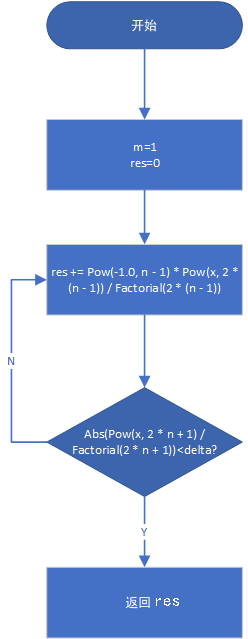
\includegraphics[width=0.32\linewidth]{src/B.png}
    \centering
    \caption{\textbf{算法 2} 泰勒多项式逼近$\sin(x)$}
\end{figure}
\subsection{误差分析}
下面分析此方法的方法误差与舍入误差。
\subsubsection{方法误差}
泰勒多项式逼近的方法误差即为其当前对应的余项
\begin{equation}
  \Delta_{2m} \leq \max|R_{2m}(x)| \leq \frac{|x|^{2m+1}}{(2m+1)!}
\end{equation}
\subsubsection{舍入误差}
假设存储误差为$\frac{1}{2}\times 10^{-k}$,则此方法的累计舍入误差为
\begin{equation}
  \delta_{2m} = |\sin(x\pm \frac{1}{2}\times 10^{-k}) - \sin(x)|
\end{equation}
使用泰勒展开并舍去高阶小量得
\begin{equation}
  \delta_{2m} \leq \left(\Sigma_{i=1}^{m} (-1)^{i-1}\frac{x^{2 i-2}}{(2 i-2) !}\right) \cdot \frac{1}{2}\times 10^{-k}
\end{equation}
\subsubsection{总误差}
考虑以上误差与计算机四则运算得累计误差得
\begin{equation}
  \Delta \leq \frac{|x|^{2m+1}}{(2m+1)!} + \left(\Sigma_{i=1}^{m} (-1)^{i-1}\frac{x^{2 i-2}}{(2 i-2) !} \right)\cdot \frac{1}{2}\times 10^{-k} + \frac{1}{2}\times 10^{-k}
\end{equation}
\subsection{计算代价}
泰勒多项式的计算次数与指定精度有着密切联系,在本任务中,迭代次数不超过 20
\subsection{收敛速度}
由于泰勒多项式逼近得算法具有试探性,每次只试探一项,但是由于下一项得阶数上升一阶,下面给出其收敛速度的大致分析,对于泰勒多项式的下一项,我们可以得到
\begin{equation}
  \alpha = \frac{\Delta_{2(m+1)}}{\Delta_{2m}} = \frac{\frac{|x|^{2(m+1)+1}}{(2(m+1)+1)!}}{\frac{|x|^{2m+1}}{(2m+1)!}} = \frac{|x|^2}{4m^2+10m+6}
\end{equation}
从而得知收敛速度$\alpha$随着计算次数的增加而减小,这符合主观感受。
\section{常微分方程}
根据$\sin(x)$函数特性可知
\begin{equation}
  {\sin}^2(x)+{\cos}^2(x)=1, \quad {\sin}'(x)={\cos}(x)
\end{equation}
得到如下常微分方程
\begin{equation}
y’=\left\{\begin{array}{l}{\sqrt{1-y^2},0 \leq x \leq 2k\pi+\frac{\pi}{2} \quad or \quad 2k\pi + \frac{3\pi}{2}} \leq x \leq 2k\pi + 2\pi \\ {-\sqrt{1-y^2},\quad 2k\pi + \frac{\pi}{2} \leq x \leq 2k\pi+\frac{3\pi}{2}}\end{array}\right.,\quad y(0)=0
\end{equation}
解此常微分方程即可求得$\sin(x)$的值。
\subsection{原理解析}
笔者使用改进欧拉法求解常微分方程
\begin{equation}
\left\{\begin{array}{l}{\bar{y}_{n+1}=y_{n}+h f\left(x_{n}, y_{n}\right)} \\ {y_{n+1}=y_{n}+\frac{h}{2}\left(f\left(x_{n}, y_{n}\right)+f\left(x_{n+1}, \bar{y}_{n+1}\right)\right)}\end{array}\right.
\end{equation}

反复迭代到指定值即可求得相应结果。
\subsection{算法流程}
算法流程参见\textbf{算法 3} 改进欧拉公式求解$\sin(x)$
\begin{algorithm}
  \caption{改进欧拉公式求解$\sin(x)$}
  \begin{algorithmic}
    \Require 待求自变量$x$与指定精度$\epsilon$
    \Ensure $x\in R$
    \begin{enumerate}
      \item 将$x$转换至标准区间
      \item 根据指定精度$\epsilon$确定步长
      \item 根据步长确定迭代次数$n$
      \item 根据改进的欧拉公式与初值反复迭代到指定次数$n$返回计算值并计算误差
    \end{enumerate}
  \end{algorithmic}
\end{algorithm}
\subsection{算法实现}
详细算法参见\href{https://github.com/Antonio-Chan/SineCalculate}{源代码}。
\subsection{程序框图}
\begin{figure}[htbp]
    \centering
    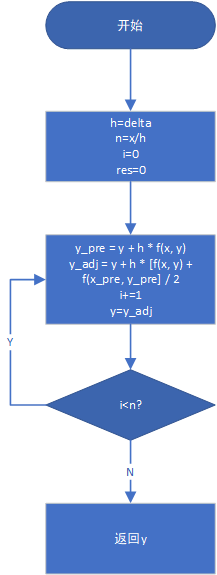
\includegraphics[width=0.3\linewidth]{src/C.png}
    \centering
    \caption{\textbf{算法 3} 改进欧拉公式求解$\sin(x)$}
\end{figure}
\subsection{误差分析}
下面分析此方法的方法误差与舍入误差。
\subsubsection{方法误差}
根据泰勒展开我们可以计算改进的欧拉法的局部截断误差为
\begin{equation}
  T_{n+1}=[y(x_{n+1})-y(x_n)]-\frac{h}{2} [y'(x_{n+1})+y'(x_n)]=-\frac{h^3}{12}y^{(3)}(x_n)+O(h^4)
\end{equation}
由此可知改进的欧拉法是二阶方法,其局部误差主项为$-\frac{h^3}{12}y^{(3)}(x_n)$

下面同理给出显示欧拉法的局部截断误差
\begin{equation}
  T_{n+1}=\frac{h^2}{2}y^{(2)}(x_n)+O(h^3)
\end{equation}
隐式欧拉法的局部截断误差
\begin{equation}
  T_{n+1}=-\frac{h^2}{2}y^{(2)}(x_n)+O(h^3)
\end{equation}

由局部截断误差我们可以计算改进的欧拉法的方法误差,即截断累积误差
\begin{equation}
  \Delta_{n+1} \leqslant\left(1+h M+\frac{h^{2}}{2} M^{2}\right) \cdot \Delta_{n}+\left(\frac{L M}{4}+\frac{T}{12}\right) \cdot h^{3}
\end{equation}
配方得
\begin{equation}
  \Delta_{n+1}+\frac{h^{2}(3 L M+T)}{6 M(h+2)} \leqslant\left(1+h M+\frac{h^{2}}{2} M^{2}\right)\left(\Delta_{n}+\frac{h^{2}(3 L M+T)}{6 M(h+2)}\right)
\end{equation}
整理得
\begin{equation}
  \Delta_{n} \leq\left(\left(1+h M+\frac{h^{2}}{2} M^{2}\right)^{n}-1\right)\cdot\frac{h^{2}(3 LM+T)}{6 M(h+2)}
\end{equation}
其中$\left|\frac{\partial f}{\partial y}(x, y)\right| \leqslant M,\quad \left|y^{(2)}(x)\right| \leqslant L,\quad \left|y^{(3)}(x)\right| \leqslant T$
\subsubsection{舍入误差}
结合改进的欧拉法表达式及局部截断误差计算方法我们可以得到舍入误差累计
\begin{equation}
  \delta_{n+1} \leqslant\left(1+h M+\frac{h^{2}}{2} M^{2}\right) \cdot \delta_{n}+\left(1+\frac{h M}{2}\right) \cdot \frac{1}{2} \times 10^{-m}
\end{equation}
配方得
\begin{equation}
  \delta_{n+1}+\frac{10^{-m}}{2hM} \leqslant\left(1+h M+\frac{h^{2}}{2} M^{2}\right)\left(\delta_{n}+\frac{10^{-m}}{2hM}\right)
\end{equation}
整理得
\begin{equation}
  \delta_{n} \leq\left(\left(1+h M+\frac{h^{2}}{2} M^{2}\right)^{n}-1 \right)\cdot\frac{10^{-m}}{2hM}
\end{equation}
其中$\left|\frac{\partial f}{\partial y}(x, y)\right| \leqslant M,\quad \left|y^{(2)}(x)\right| \leqslant L,\quad \left|y^{(3)}(x)\right| \leqslant T$,$m$为指定的存储位数。
\subsubsection{总误差}
考虑以上误差与计算机四则运算得累计误差得
\begin{equation}
  \Delta_{T_n} \leq\left(\left(1+h M+\frac{h^{2}}{2} M^{2}\right)^{n}-1 \right)\cdot\left(\frac{10^{-m}}{2hM}+\frac{h^{2}(3 LM+T)}{6 M(h+2)}\right)+\frac{1}{2}\cdot 10^{-m}
\end{equation}
在此方法中,可以确定
\begin{equation}
  \quad L=1,\quad T=1,\quad \left|\frac{\partial f}{\partial y}(x, y)\right| = \left|\frac{-y}{\sqrt{1-y^2}}\right| \leqslant 1 = M\quad x\in[0,\ \frac{\pi}{4})
\end{equation}
\subsection{计算代价}
改进的欧拉法的计算次数与指定精度有着密切联系,迭代次数不超过$\frac{1}{\epsilon}$
\subsection{收敛速度}
根据局部截断误差的递推公式我们可以给出其收敛速度的大致分析
\begin{equation}
  \alpha = \frac{\Delta_{n+1}}{\Delta_{n}} = 1+h M+\frac{h^{2}}{2} M^{2}
\end{equation}
从而得知收敛速度$\alpha$为一常数,线性收敛。
\section{实验结果}
以下是实验结果及分析。
\subsection{程序使用说明}
\begin{figure}[htbp]
    \centering
    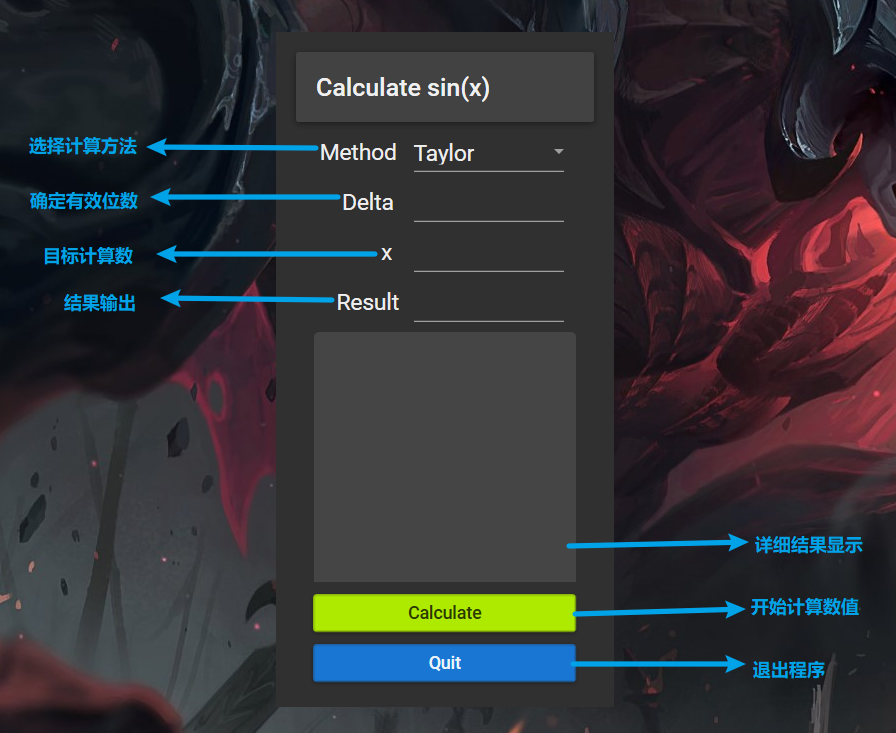
\includegraphics[width=0.8\linewidth]{src/D.png}
    \centering
    \caption{程序使用说明示意图}
\end{figure}

注意:请双击Release文件夹下的SineNumericalAnalysis.exe文件运行程序,$Delta$项输入为正整数$m$,其计算精度为$10^{-m}$。
\subsection{实验结果分析}

\begin{table}[htbp]
  \centering
  \caption{数值算法收敛性比较(输入$x=0.5$,比较项目为迭代次数)}
  \begin{tabular}{p{80pt}<{\centering}|p{80pt}<{\centering}|p{80pt}<{\centering}|p{80pt}<{\centering}}
  \Xhline{1.0pt}
  精度($\frac{1}{2}\times10^{-k}$) & Euler法 & Taylor展开 & Newton法求根 \\ \Xhline{1.0pt}
  1 & 1 & 1 & 2 \\ \hline
  2 & 57 & 2 & 3 \\ \hline
  3 & 57 & 2 & 4 \\ \hline
  4 & 5708 & 3 & 4 \\ \hline
  5 & 5708 & 3 & 4 \\ \hline
  6 & 570796 & 4 & 5 \\ \hline
  7 & 570796 & 4 & 5 \\ \hline
  8 & 57079633 & 4 & 5 \\ \hline
  9 & 57079633 & 5 & 5 \\ \hline
\end{tabular}
\end{table}

\begin{table}[htbp]
  \centering
  \caption{数值算法计算代价比较(精度$\frac{1}{2}\times 10^{-6}$,比较项目为计算时间,单位为毫秒)}
  \begin{tabular}{p{80pt}<{\centering}|p{80pt}<{\centering}|p{80pt}<{\centering}|p{80pt}<{\centering}}
  \Xhline{1.0pt}
  输入$x$ & Euler法 & Taylor展开 & 系统Math.Sin() \\ \Xhline{1.0pt}
  -10 & 292.4622 & 0.0042 & 0.0003 \\ \hline
  -7.5 & 174.1181 & 0.004 & 0.0003 \\ \hline
  -5 & 123.683 & 0.0043 & 0.0003 \\ \hline
  -3.1416 & 0.0067 & 0.0027 & 0.0003 \\ \hline
  -1.5708 & 0.0055 & 0.003 & 0.0003 \\ \hline
  -1 & 268.0678 & 0.0065 & 0.0003 \\ \hline
  -0.5 & 304.2473 & 0.0049 & 0.0003 \\ \hline
  0 & 0.0026 & 0.0031 & 0.0003 \\ \hline
  0.5 & 272.6894 & 0.0053 & 0.0003 \\ \hline
  1 & 271.035 & 0.0055 & 0.0003 \\ \hline
  1.5708 & 0.0049 & 0.0031 & 0.0003 \\ \hline
  3.1416 & 0.0074 & 0.0035 & 0.0003 \\ \hline
  5 & 132.1457 & 0.0049 & 0.0003 \\ \hline
  7.5 & 170.8583 & 0.3234 & 0.0003 \\ \hline
  10 & 269.9762 & 0.0054 & 0.0003 \\ \hline
\end{tabular}
\end{table}

在收敛性比较中我们可以看出,由于Taylor展开是直接代入已有公式,所以其迭代步数极少,同时我们也可以看出,Newton法求平方根的迭代次数也很少,这显示出其优越的收敛性及稳定性,但是Euler法则会随着精度要求的增加而显著增加迭代次数,可见欧拉法相较于Taylor法更加消耗计算资源。

在计算代价的比较中我们可以看到计算代价与迭代步骤是正相关的,迭代次数越多计算时间越长,从实际运行结果我们看到距离函数值为0或1的点越近,Euler计算速度越快,其他点计算速度均在几百毫秒左右,这说明Euler法是初值敏感的,初值确定的好,其收敛速度也较快,从表中的对比我们不难看出系统自带的函数计算速度与Taylor展开相接近,我们可以做出合理猜想,即系统中的$sin(x)$函数的计算采用的是多项式逼近的方法。

\begin{figure}[htbp]
  \begin{minipage}[htbp]{0.4\linewidth}
    \centering
    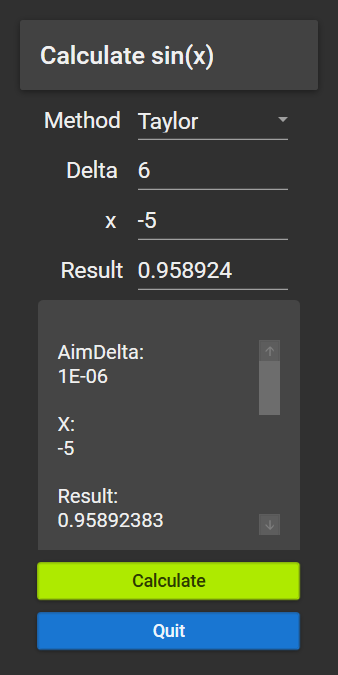
\includegraphics[width=0.8\linewidth]{src/E.png}
    \caption{Taylor}
    \centering
  \end{minipage}
  \hfill
  \begin{minipage}[htbp]{0.5\linewidth}
    Taylor计算详细结果
    \begin{itemize}
      \item AimDelta: 1E-06
      \item X: -5
      \item Result: 0.95892383
      \item StorageAcc: 1E-15
      \item IterationTimes: 11
      \item MethodDelta: 4.6112182E-07
      \item TruncationDelta: 2.8366421E-16
      \item CalDelta: 4.6112182E-07
    \end{itemize}
  \end{minipage}
\end{figure}

\begin{figure}[htbp]
  \begin{minipage}[htbp]{0.4\linewidth}
    \centering
    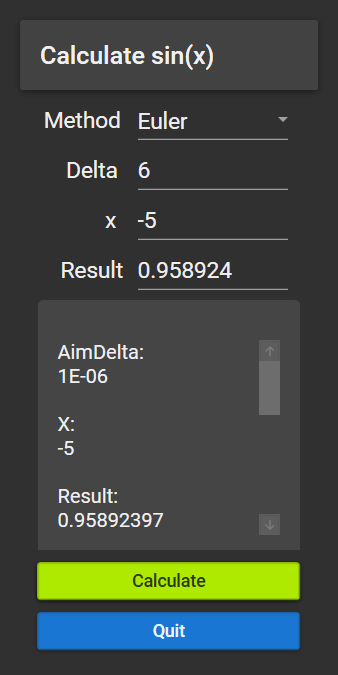
\includegraphics[width=0.8\linewidth]{src/F.png}
    \caption{Euler}
    \centering
  \end{minipage}
  \hfill
  \begin{minipage}[htbp]{0.5\linewidth}
    Euler计算详细结果
    \begin{itemize}
      \item AimDelta: 1E-06
      \item X: -5
      \item Result: 0.95892397
      \item StorageAcc: 1E-15
      \item IterationTimes: 5000000
      \item MethodDelta: 1.6037019E-12
      \item TruncationDelta: 7.6016178E-09
      \item CalDelta: 7.603222E-09
    \end{itemize}
  \end{minipage}
\end{figure}

\section{参考文献}
[1]李庆扬,王能超等.《数值分析》[M].北京:清华大学出版社,2008:51-66,212-227,279-285.
\end{document}
